\chapter{物理疑难杂症}
\section{真空态与绘景}
\section{轴子和伸缩子}\label{A.2}
文献里经常会碰到这俩概念,虽然是作为暗物质的候选者,应当是唯象的关注对象,但形式理论中也处处见他们的身影。
\subsection{轴子(Axion)}
为了解释轴子的概念,先介绍\textbf{强CP问题}。这首先要从QCD的手征反常说起,后面会用到其中建立起来的一些工具。

\subsection{轴子电动力学}

\subsection{伸缩子(Dilaton)}
不少人也把它翻译成胀子。
\section{费曼规则}
这一节我不想讨论任何有关费曼规则推导的问题,只是通过拉氏量看出费曼规则,重点在对常用费曼规则的整理。本节讨论的都是动量空间的费曼规则,也就是把顶点的动量守恒都已经积成$\delta$函数了,计算上大家都是用的动量空间,因为更方便。
\subsection{标量场和矢量场}
这部分的费曼规则是基操,非常简单没有任何需要多说的,除了复标量场,由于和费米子又点想,留到下一小节再进行讨论。整体的费曼规则见图\ref{fig.A.3.2}(不包含顶角)。
\begin{figure}[htbp]
	\centering
	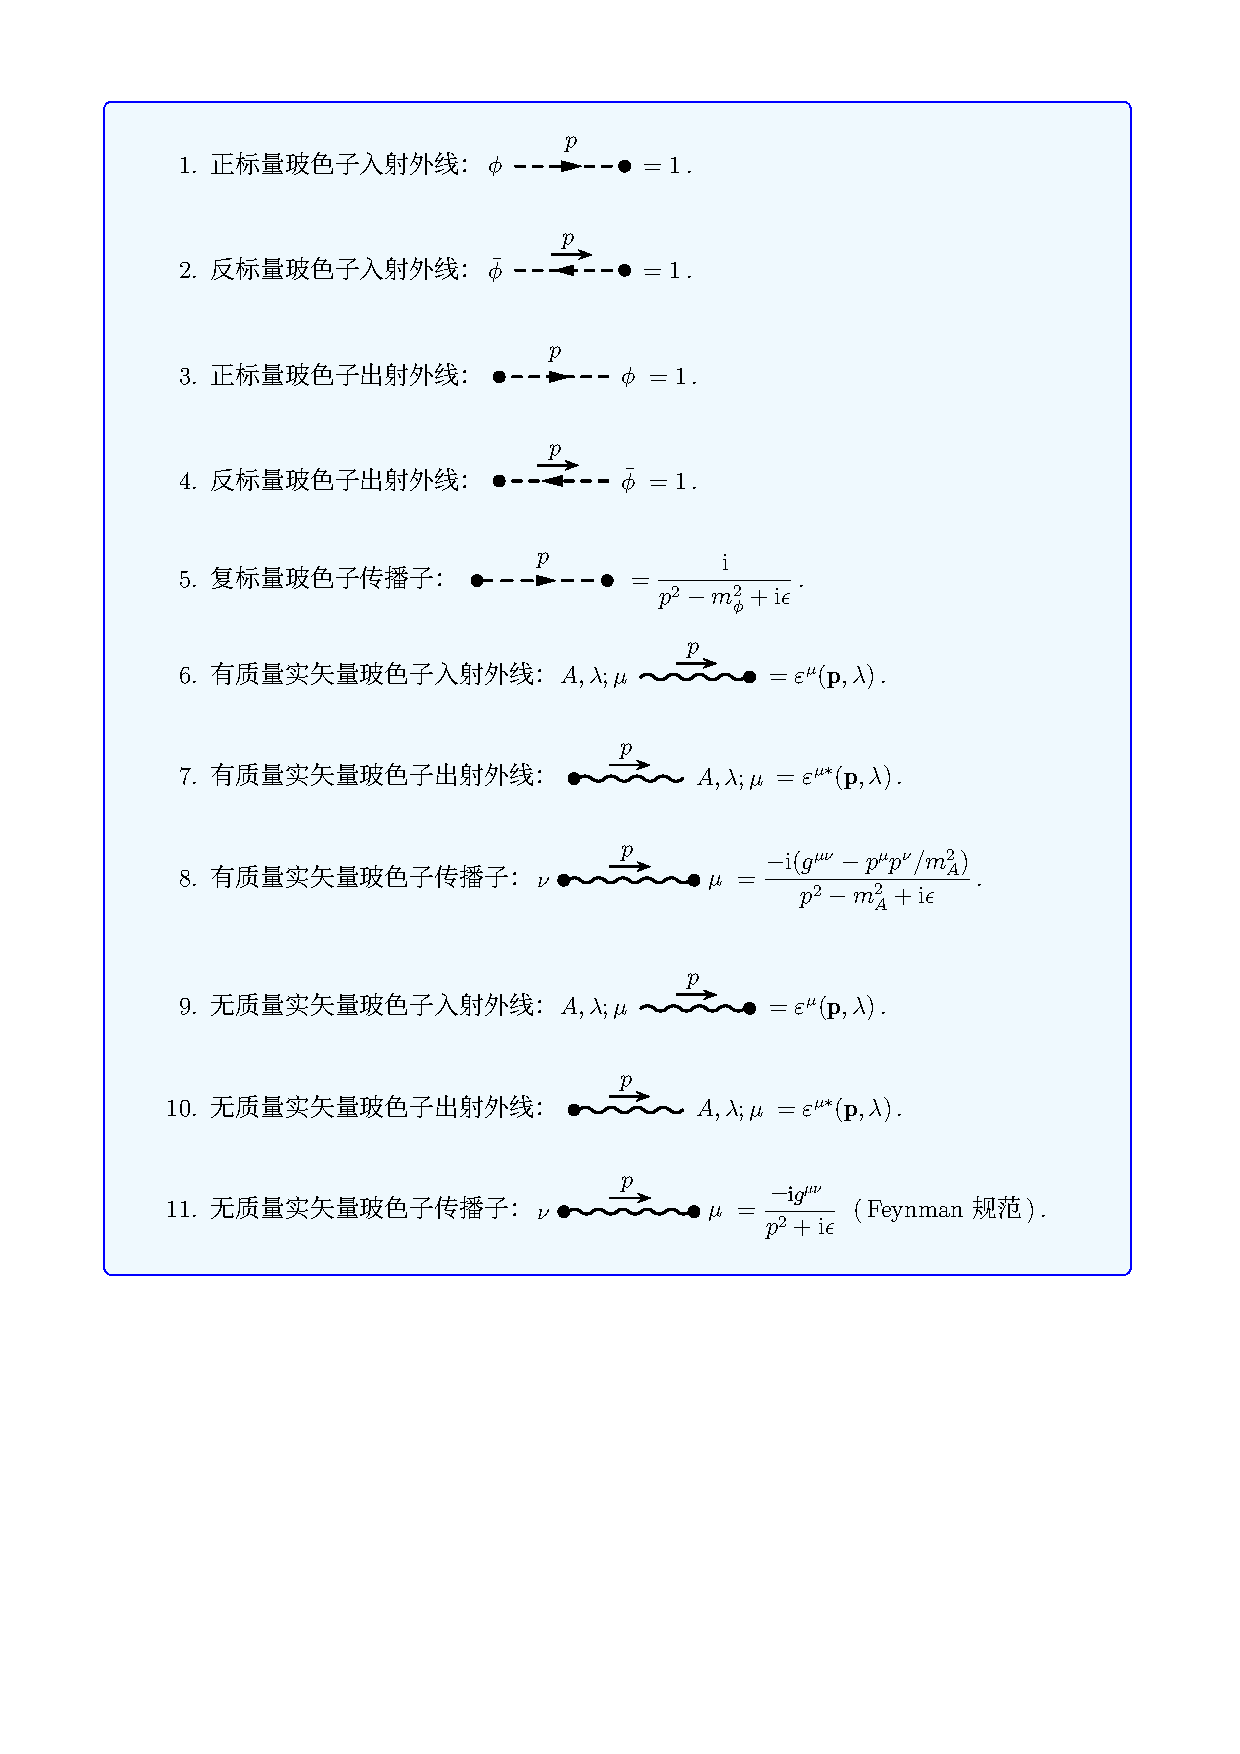
\includegraphics[width=\linewidth]{figs/fig20.pdf}
	\label{fig.A.3.2}
	\caption{一般内外线费曼规则}
\end{figure}
\subsection{Dirac和Majorana费米子}
这应该是费曼规则里最麻烦的部分,主要就是要分清三个箭头:动量箭头、$U(1)$箭头和费米子流箭头。很多教科书写费曼规则总是引入更少的箭头,反而搞一堆正负号规则,如果讨论的是标量场或者是矢量场,这没太大问题,但是对于旋量场,我认为最清楚的方式就是多画一些箭头。我们考虑下面的具有$CP$对称性的复标量场和Dirac场$\psi$以及Majorana场$\chi$的耦合:\footnote{这类费曼图构造可以更加复杂,尤其是涉及到费米子数破坏的理论。}
\begin{equation}\label{A.3.1}
	\mathcal{L}=(\partial^\mu\phi^\dagger)\partial_\mu\phi-m_\phi^2\phi^\dagger\phi+\bar{\psi}(\mathrm{i}\gamma^\mu\partial_\mu-m_\psi)\psi+\frac12\bar{\chi}(\mathrm{i}\gamma^\mu\partial_\mu-m_\chi)\chi+\mathcal{L}_\mathrm{int}
\end{equation}
从拉氏量可以看出我们选取的是$(+,-,-,-)$的度规\footnote{无论什么度规选取,都要保证对时间偏导的哪一个动能项是正的},原因是我本节费曼规则的图全部是抄的余钊焕老师讲义。这里相互作用项为:
\begin{equation}
	\mathcal{L}_\mathrm{int}=\kappa\phi^\dagger\bar{\chi}P_\mathrm{R}\psi+\kappa^*\phi\bar{\psi}P_\mathrm{L}\chi 
\end{equation}
选取$\kappa\in\mathbb{R}$,并引入记号$\Gamma_1=P_\mathrm{R},\quad\Gamma_2=P_\mathrm{L}$,这时为了突出下面的结果与$\Gamma_{1,2}$具体形式无关:
\begin{equation}
	\mathcal{L}_{\mathrm{int}}=\kappa(\phi^\dagger\bar{\chi}\Gamma_1\psi+\phi\bar{\psi}\Gamma_2\chi)
\end{equation}
其费曼规则如图\ref{fig.A.3.1}所示。下面我们来逐一解释每一项,并给出一些例子。
\begin{figure}[htbp]
	\centering
	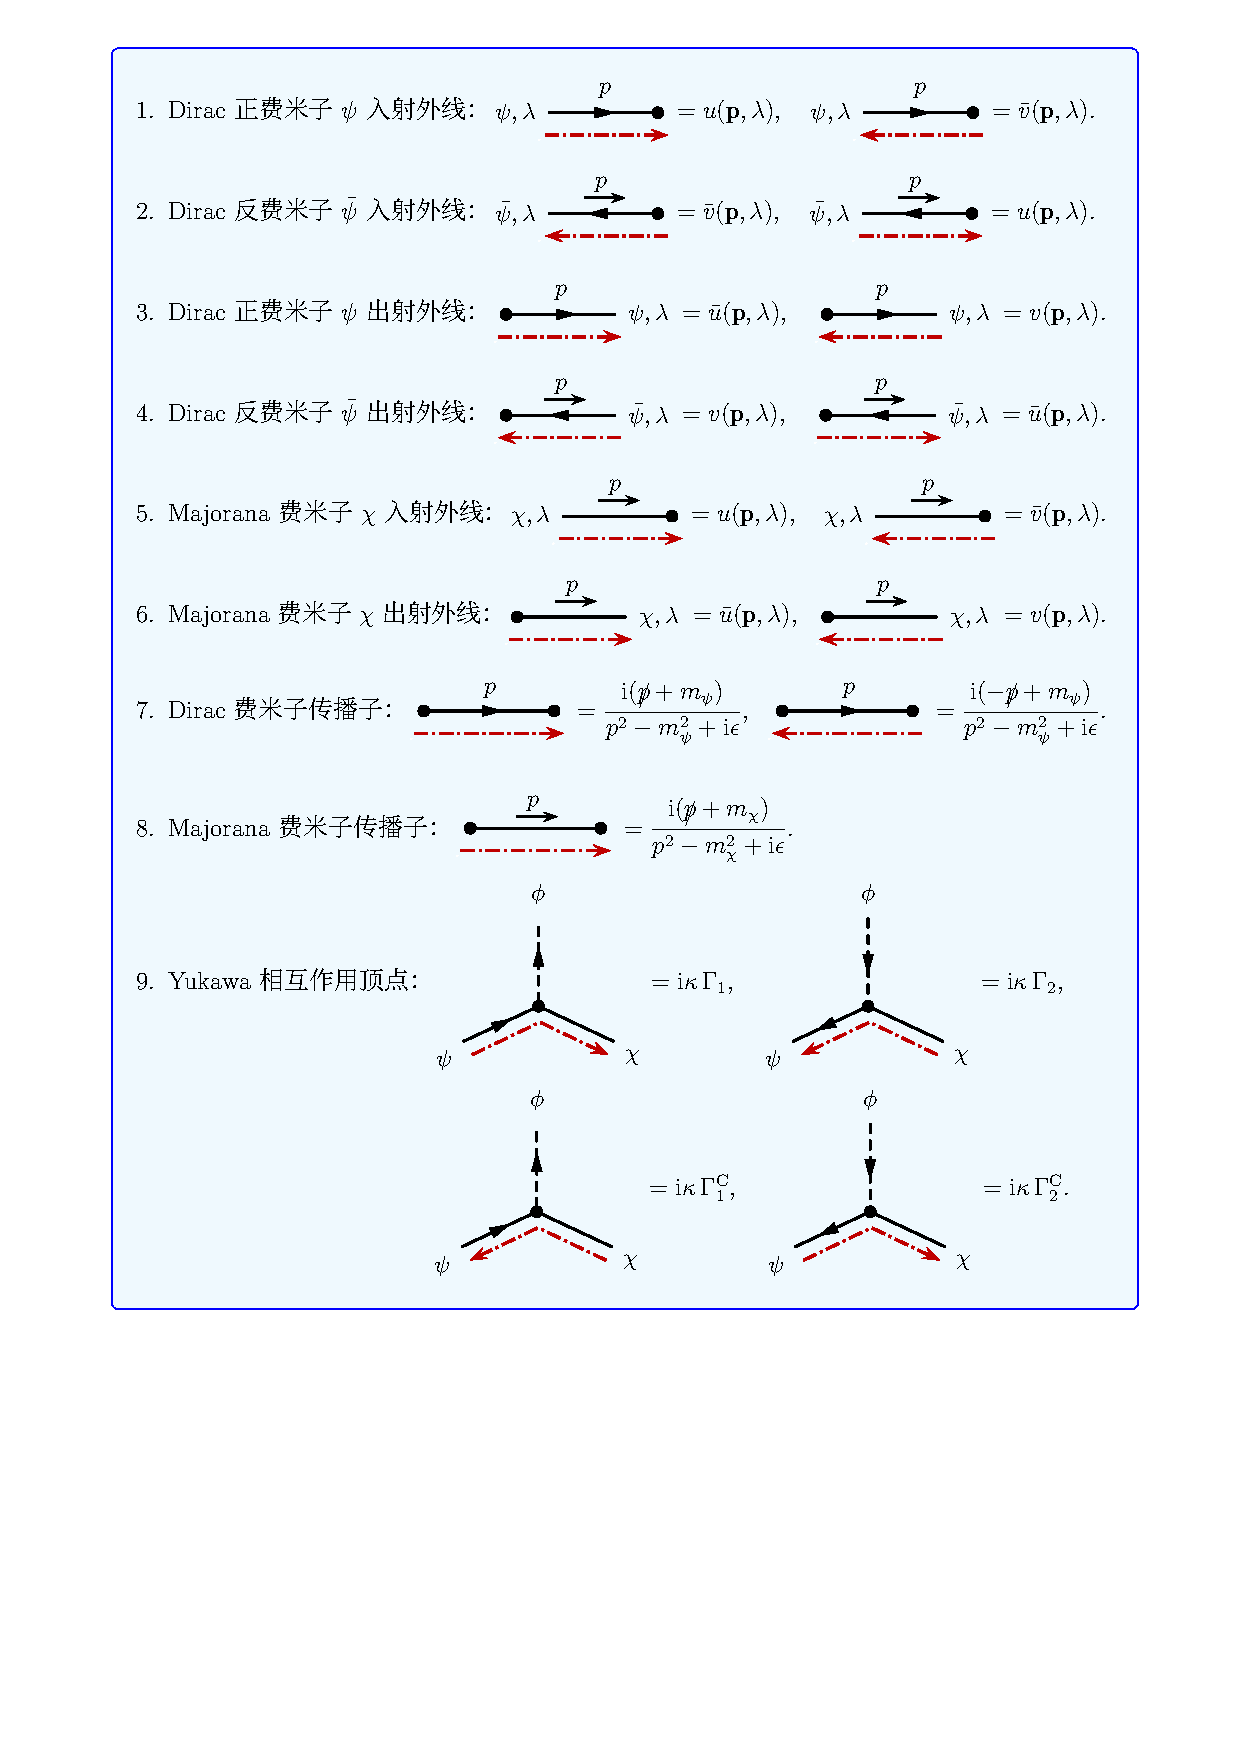
\includegraphics[width=\linewidth]{figs/fig19.pdf}
	\caption{\ref{A.3.1}的费曼规则}
	\label{fig.A.3.1}
\end{figure}

首先注意到图中出现了三种箭头,最上面的是动量箭头,标记的是粒子动量的正方向,根据这一点去要求每个顶点动量守恒,另外它还标记了粒子是入射还是出射,如果箭头流入节点,就是入射,流出就是出射;中间的是$U(1)$箭头,这是因为Dirac有正反两种不同的粒子所特有的,Majorana粒子就没有,这个箭头和动量箭头一起用来标记是正粒子还是反粒子,如果同向则为正,反向为反。这样做的好处是你不需要引入一个时间轴,来区分哪些粒子是正,哪些是反,哪些是出射,哪些是入射;最下面的箭头是费米子流,注意这个箭头是画在一整个费米子线段构成的折线上的,也就是说在每个费米子流线上,每个小段的流向一致,这是由于理论中有Majorana费米子,由于Majorana正反粒子相同,但是计算又必须引入一个方向所特别引入的一个附加规则。最后注意到有些图上我们把动量箭头和$U(1)$箭头合二为一了,这意味着两者是同向的,比如费米子内线我们就把两者取成一个方向。

再看顶角,这种复标量场和旋量场,根据耦合项读费曼规则,始终记住指向节点的表示$\phi\backslash\psi$,指出节点的是$\phi^{\dagger}\backslash\bar\psi$。Majorana耦合要根据费米子流来,复杂一点。复标量场的内外线规则可见\ref{fig.A.3.2},除了是玻色子,不需要引入费米子流来分清共轭、相对符号这些,其它和上一段讲的都一样。

费曼规则中还涉及到了电荷反演,下面是一些公式总结:
\begin{equation}
	\mathcal{C}^\mathrm{T}=\mathcal{C}^\dagger=\mathcal{C}^{-1}=-\mathcal{C},\quad
	\Gamma^{\mathrm{C}}\equiv\mathcal{C}^{-1}\Gamma^{\mathrm{T}}\mathcal{C},\quad v(\mathbf{p},\lambda)=\mathcal{C}\bar{u}^{\mathrm{T}}(\mathbf{p},\lambda),\quad u(\mathbf{p},\lambda)=\mathcal{C}\bar{v}^{\mathrm{T}}(\mathbf{p},\lambda)
\end{equation}

另外我们这都是对树图的,对于圈图,还有一些来自圈的对称因子没有抵消殆尽,而且每个圈动量都要带来积分$\int\frac{d^4p}{(2\pi)^4}$,然后用维数正规化这些进行计算。而且\textbf{费米子圈会带来一个额外的符号},$\gamma$矩阵也要随之取迹。下面以$\chi\chi\to\psi\bar{\psi}$的计算为例。只考虑树图阶的贡献,首先第一步是根据费曼规则含有的顶点绘制出所有的不等价的费曼图,有全同粒子要对全同粒子动量标号后绘制,如图\ref{fig.A.3.3}
\begin{figure}[htbp]
	\centering
	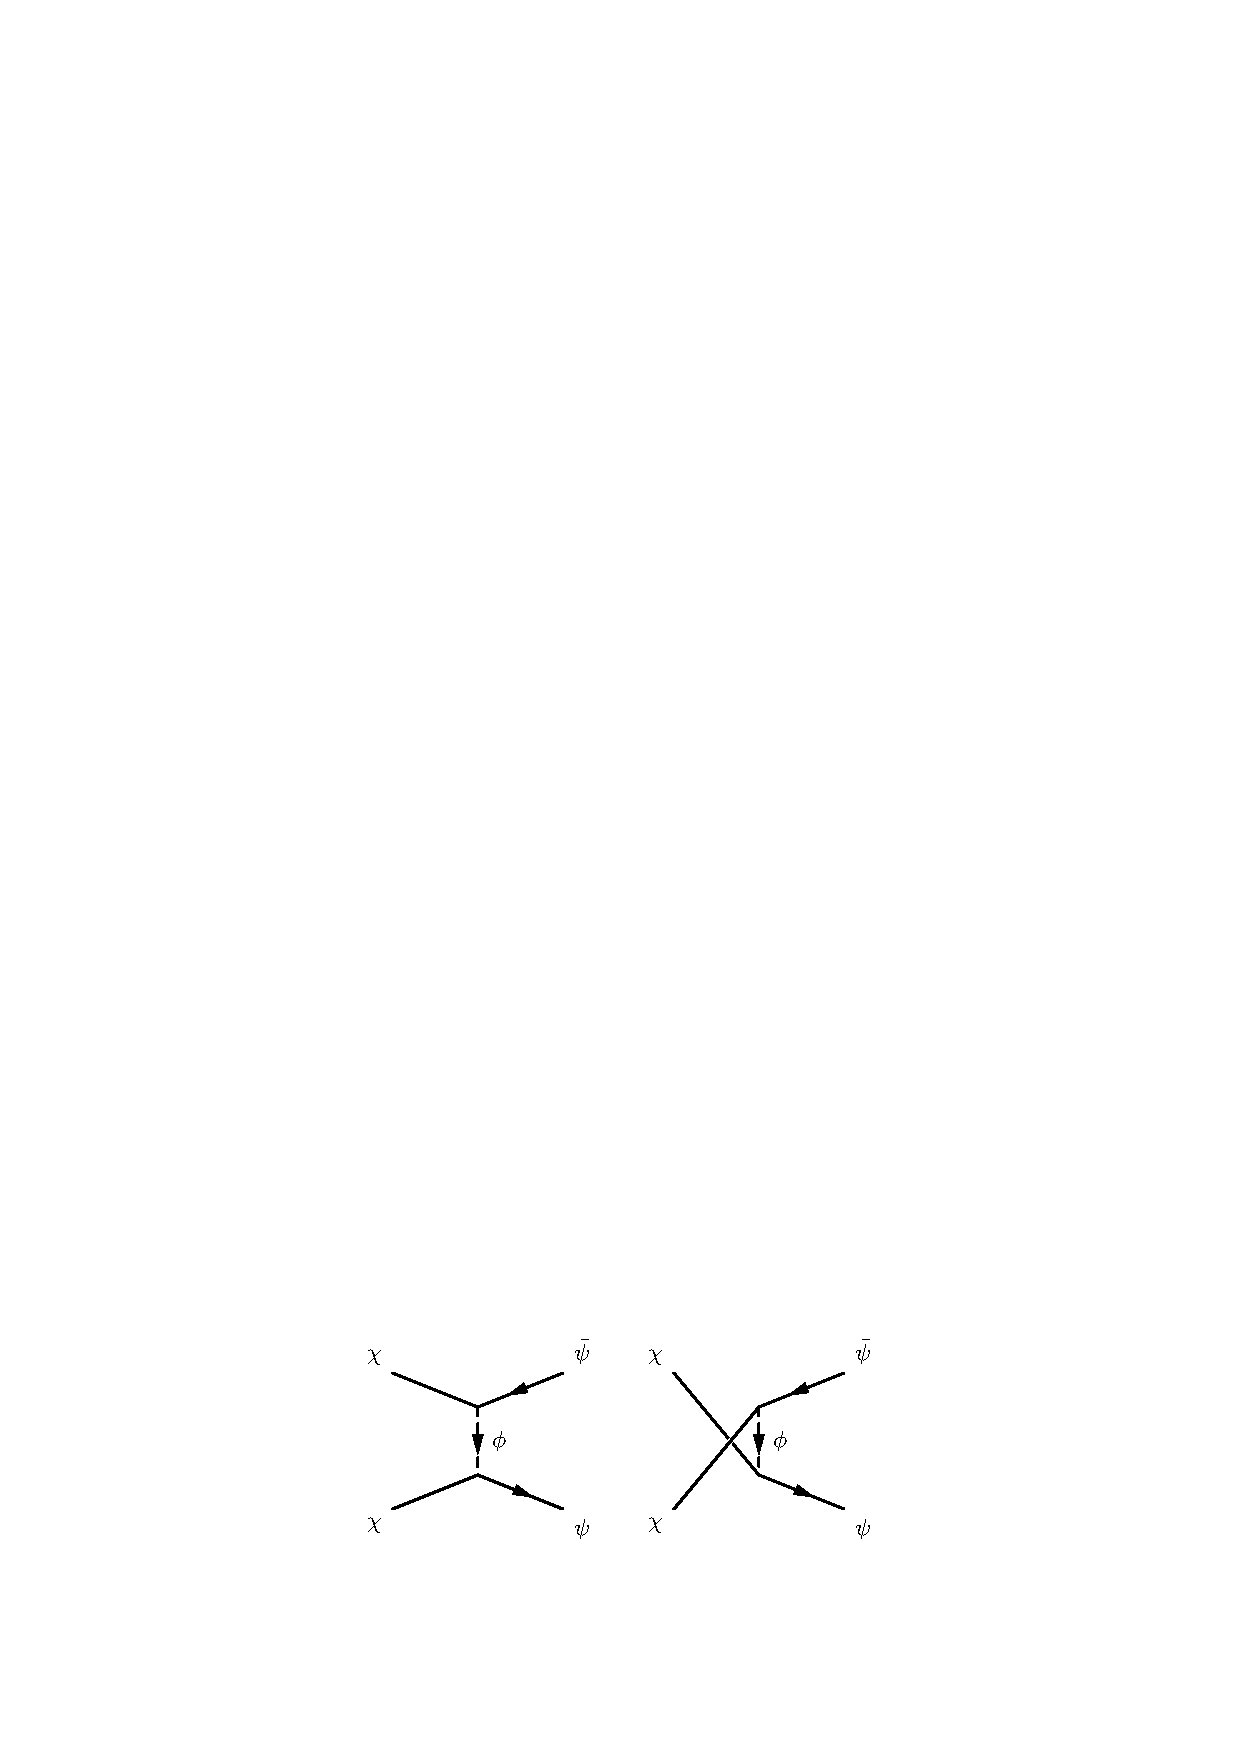
\includegraphics{figs/fig21.pdf}
	\caption{$\chi\chi\to\psi\bar{\psi}$散射树图}
	\label{fig.A.3.3}
\end{figure}

注意,我们并没有绘制费米子流,实际上图\ref{fig.A.3.2}给出的是两套等价的费曼规则,计算时我们需要人为地指定费米子流方向,然后逆着每个费米子流去写相应的项,无论怎么选费米子流,得到的结果都是一样的\footnote{也就是说费米子流本身并不带来任何拓扑不等价的图,他只是为了计算的方便性引入的。}。这可以从费曼规则里面的顶点看出来。观察\ref{fig.A.3.2}的第九项第一列,动量箭头假设都是从左到右。如果我们反转某个费米子流箭头,其它两个箭头不变,那么顶点项会从${\bar u}_\chi \Gamma_1 u_\psi \to{\bar v}_{\psi} \Gamma_1^C{{v}}_\chi$,根据下面的式子:
\begin{equation}\label{A.5}
		{\bar u}_\chi \Gamma_1 u_\psi= v_\chi^{\mathrm{T}}\mathcal{C} \mathcal{C}^{-1}\Gamma_1^\mathrm{T} \mathcal{C}\mathcal{C}\bar{v}^{\mathrm{T}}_{\psi}=-\left(v_\chi^{\mathrm{T}}\Gamma_1^\mathrm{T} \bar{v}^{\mathrm{T}}_{\psi}\right)^{\mathrm{T}}
		=-{\bar v}_{\psi} \Gamma_1^C{{v}}_\chi
\end{equation}

所以改变一个费米子流和加上一个负号是等价的,这在后面考虑相对符号时非常有用,把相对符号考虑进来后会发现无论你怎么取费米子流方向,最终把所有的图加起来后,只会整体让振幅差个正负号,这是无所谓的。

比如下面的选取:
\begin{equation}
	\begin{aligned}
		\mathrm{i}\mathcal{A}_{t}&=\parbox[c]{3cm}{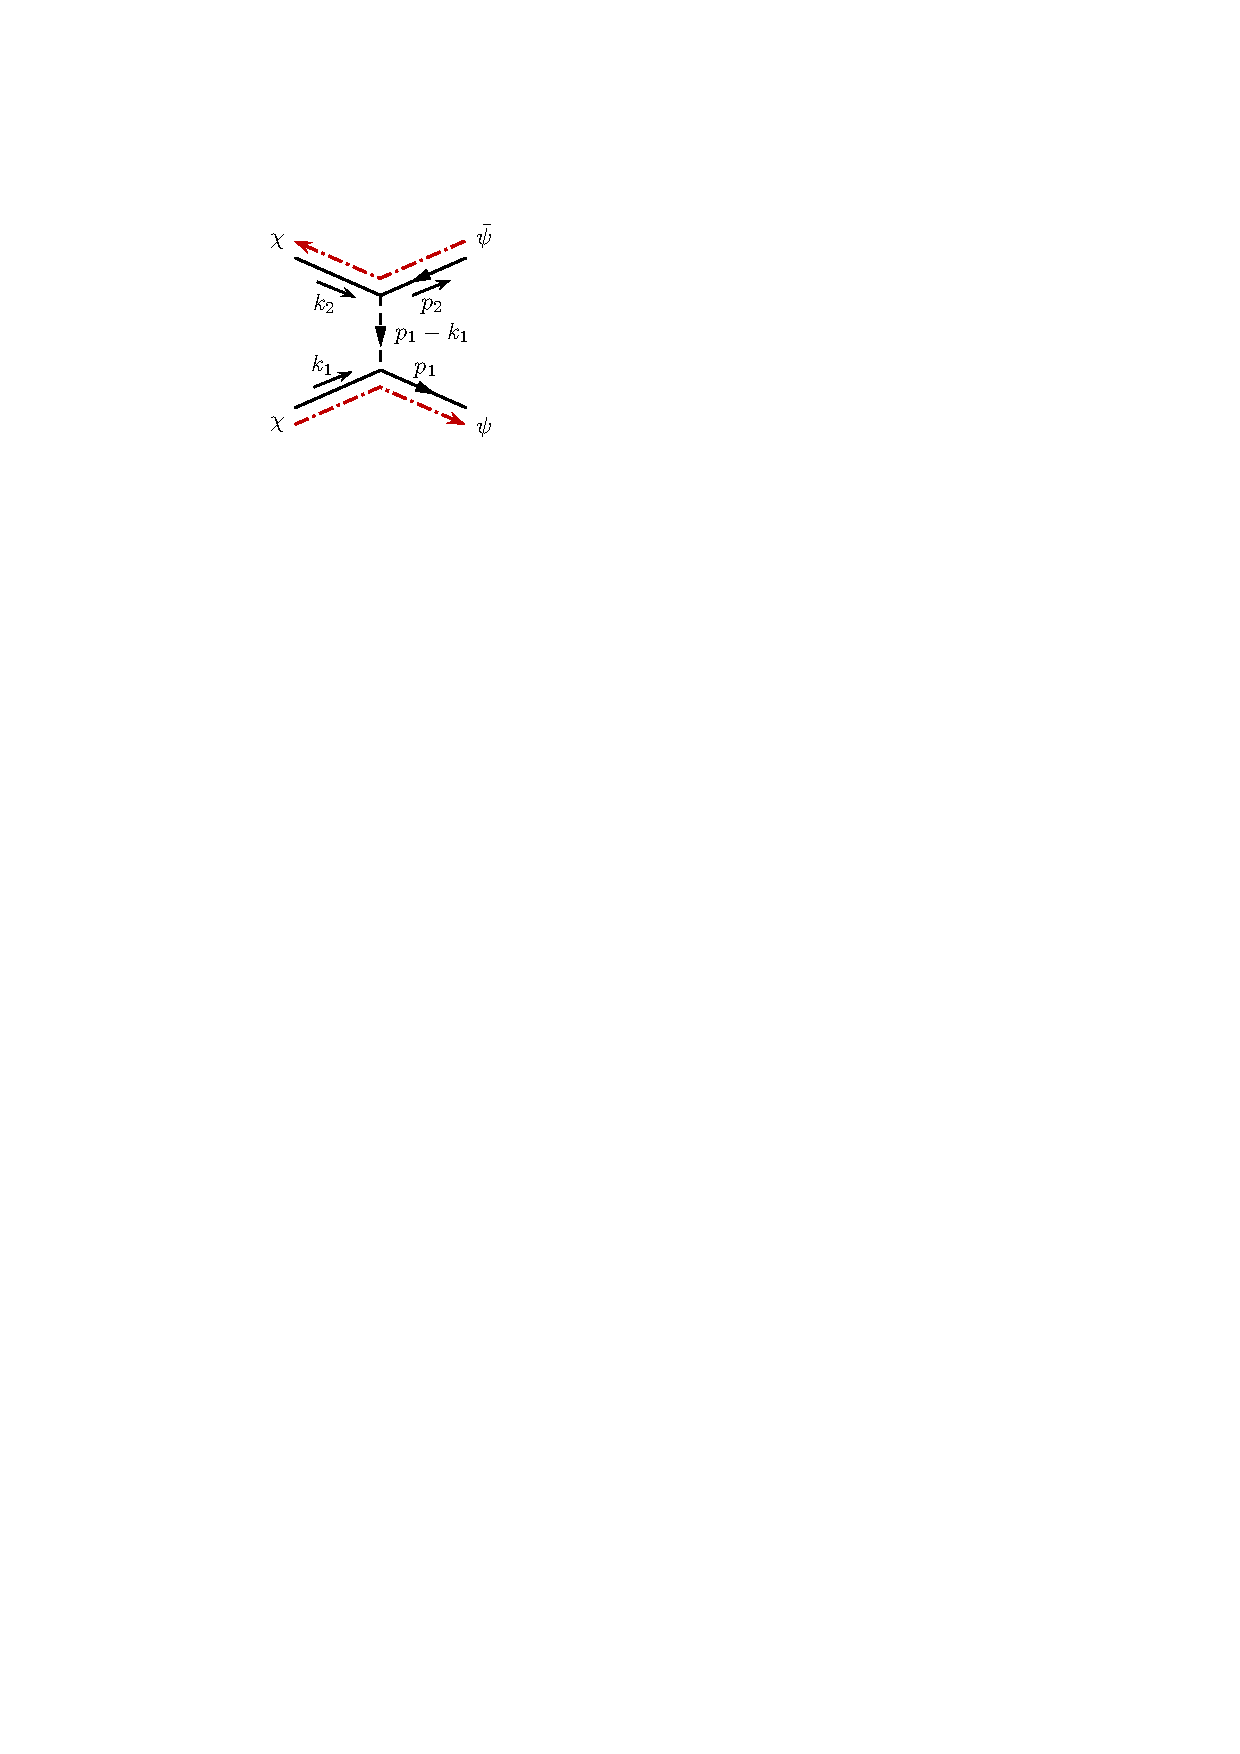
\includegraphics[width=3cm]{figs/fig22.pdf}}=\bar{u}(p_1)(\mathrm{i}\kappa\Gamma_2)u(k_1)\frac{\mathrm{i}}{(p_1-k_1)^2-m_\phi^2}\bar{v}(k_2)(\mathrm{i}\kappa\Gamma_1)v(p_2)\\
		&=-\frac{\mathrm{i}\kappa^2}{t-m_\phi^2}\bar{u}(p_1)\Gamma_2u(k_1)\bar{v}(k_2)\Gamma_1v(p_2)
	\end{aligned}
\end{equation}
\begin{equation}
	\begin{aligned}
		\mathrm{i}\mathcal{A}_{u}&=\parbox[c]{3cm}{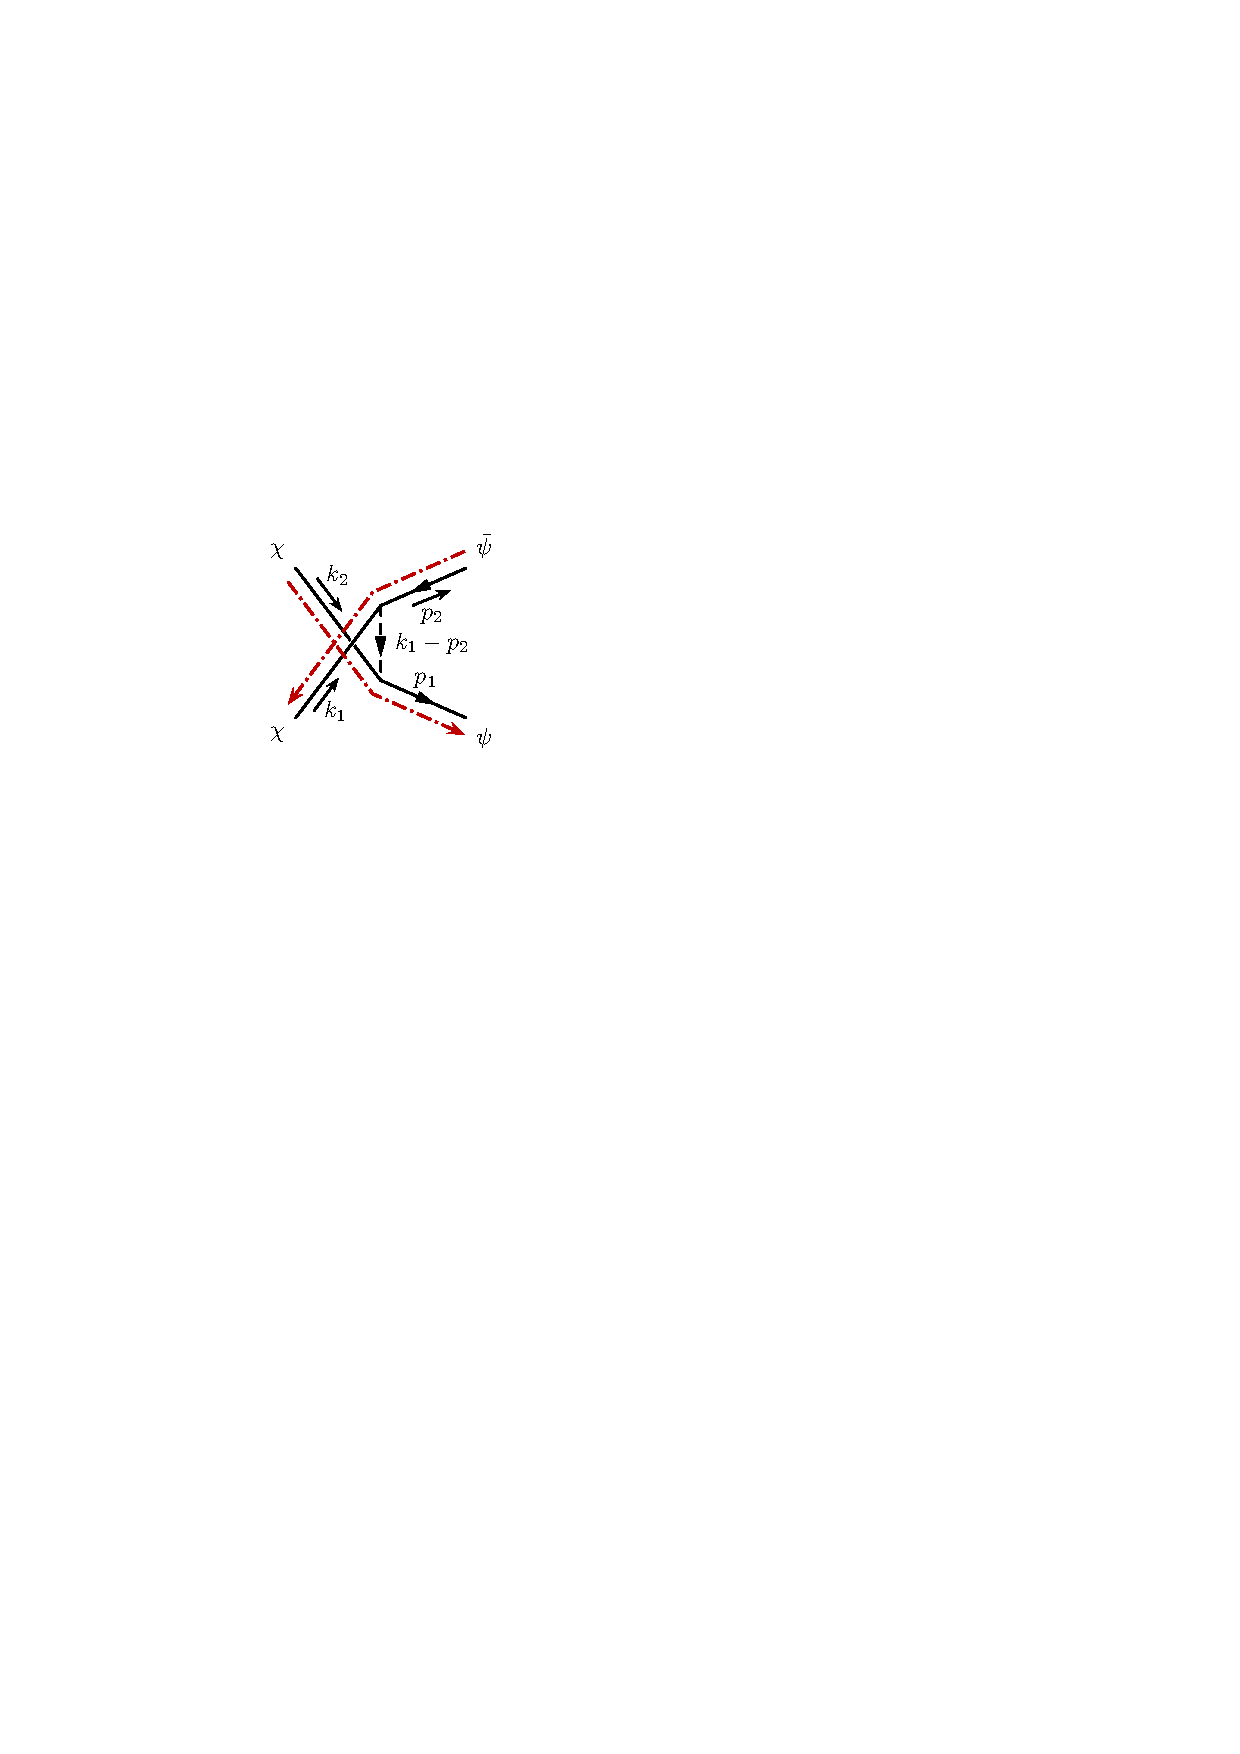
\includegraphics[width=3cm]{figs/fig23.pdf}}=\bar{v}(k_1)(\mathrm{i}\kappa\Gamma_1)v(p_2)\frac{\mathrm{i}}{(k_1-p_2)^2-m_\phi^2}\bar{u}(p_1)(\mathrm{i}\kappa\Gamma_2)u(k_2)\\
		&=-\frac{\mathrm{i}\kappa^2}{u-m_\phi^2}\bar{v}(k_1)\Gamma_1v(p_2)\bar{u}(p_1)\Gamma_2u(k_2)
	\end{aligned}
\end{equation}
费米子还有一个非常麻烦的地方就是不同费曼图贡献存在相对符号,如果一个过程只有一个图有贡献倒无所谓,但是多个图贡献就会导致干涉。这种符号的处理可以按照下面的规则:
\begin{description}
	\item[相对符号判断:] 我们要做的事情就是把所有的费曼图按照标准画法重新画一遍,可以理解成把顶点转动一下,由于我们的记号不需要引入时间轴来区分正反粒子和出入射粒子,所以不用担心弄混。首先把费曼图画成所有的费米子线都在水平方向,而且费米子流都是从左到右,左端的粒子从上到下都是一样的标号(随便取一个为标准,不同的选取只会导致振幅整体差一个正负号),这里标号就是说的动量的标号。最后看右端的粒子标号,如果两个图右端粒子的标号相差一个奇置换,则相对符号为负,否则为正。
	
	比如上面两个式子的费曼图画成标准形式为\ref{fig.A.6},注意无论你怎么画都不能把两个图的左端粒子变成一样的,所以这个时候就要引入反转费米子流箭头等价于把原先的图加个正负号。所以我们可以选择同时反转两幅图最上面的费米子流,由于都加个负号所以相对符号仍旧为正。这个时候就可以把图画成标准形式了,不难发现两幅图的右端相差一个奇置换,所以相对负号为负。
\end{description}
\begin{figure}[htbp]
	\centering
	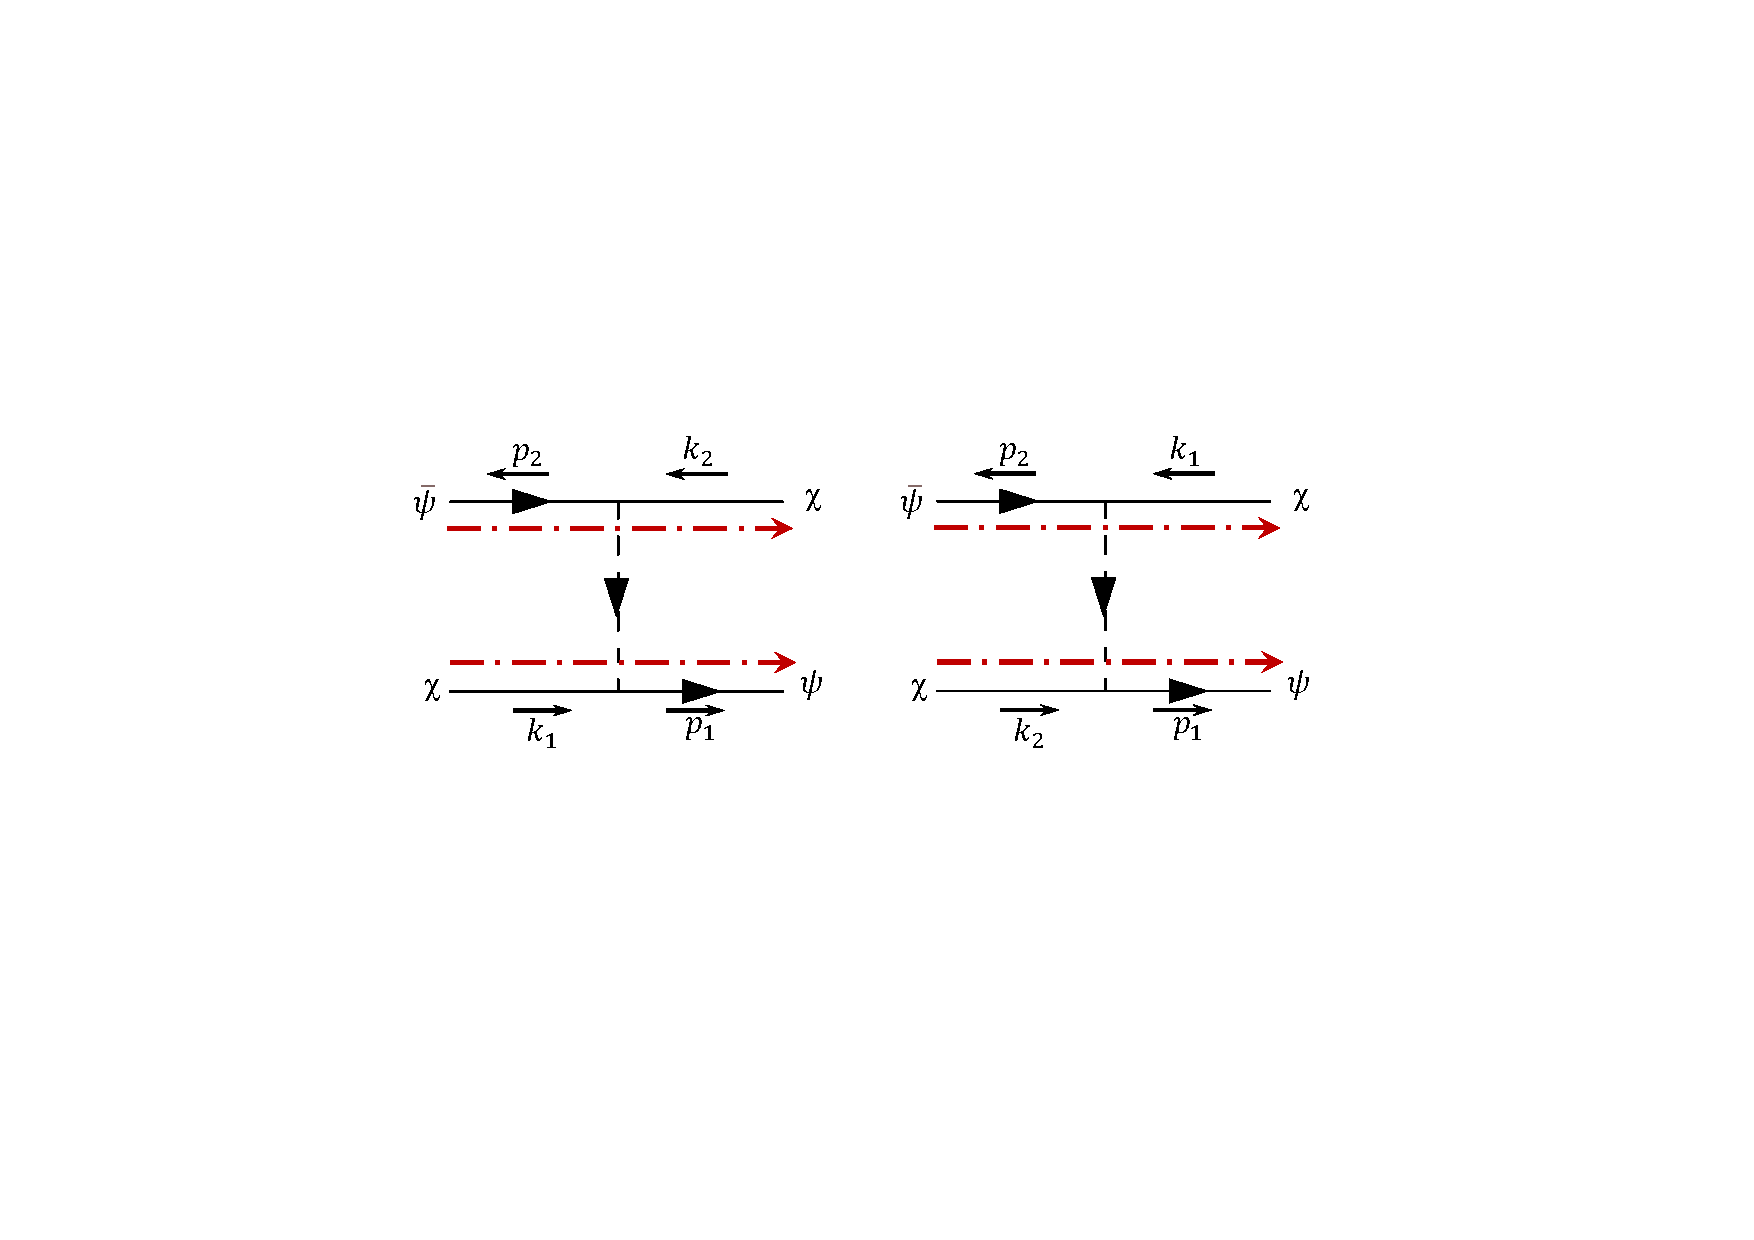
\includegraphics[width=0.6\linewidth]{figs/fig24.pdf}
	\caption{费曼图的标准画法}
	\label{fig.A.6}
\end{figure}
所以容易判断上面的两项应该相减,$\mathrm{i}\mathcal{A}=\mathrm{i}\mathcal{A}_t-\mathrm{i}\mathcal{A}_u$。还有下面的费米子流选取方式:
\begin{equation}
	\begin{aligned}
		\mathrm{i}\tilde{\mathcal{A}}_t&=\parbox[c]{3cm}{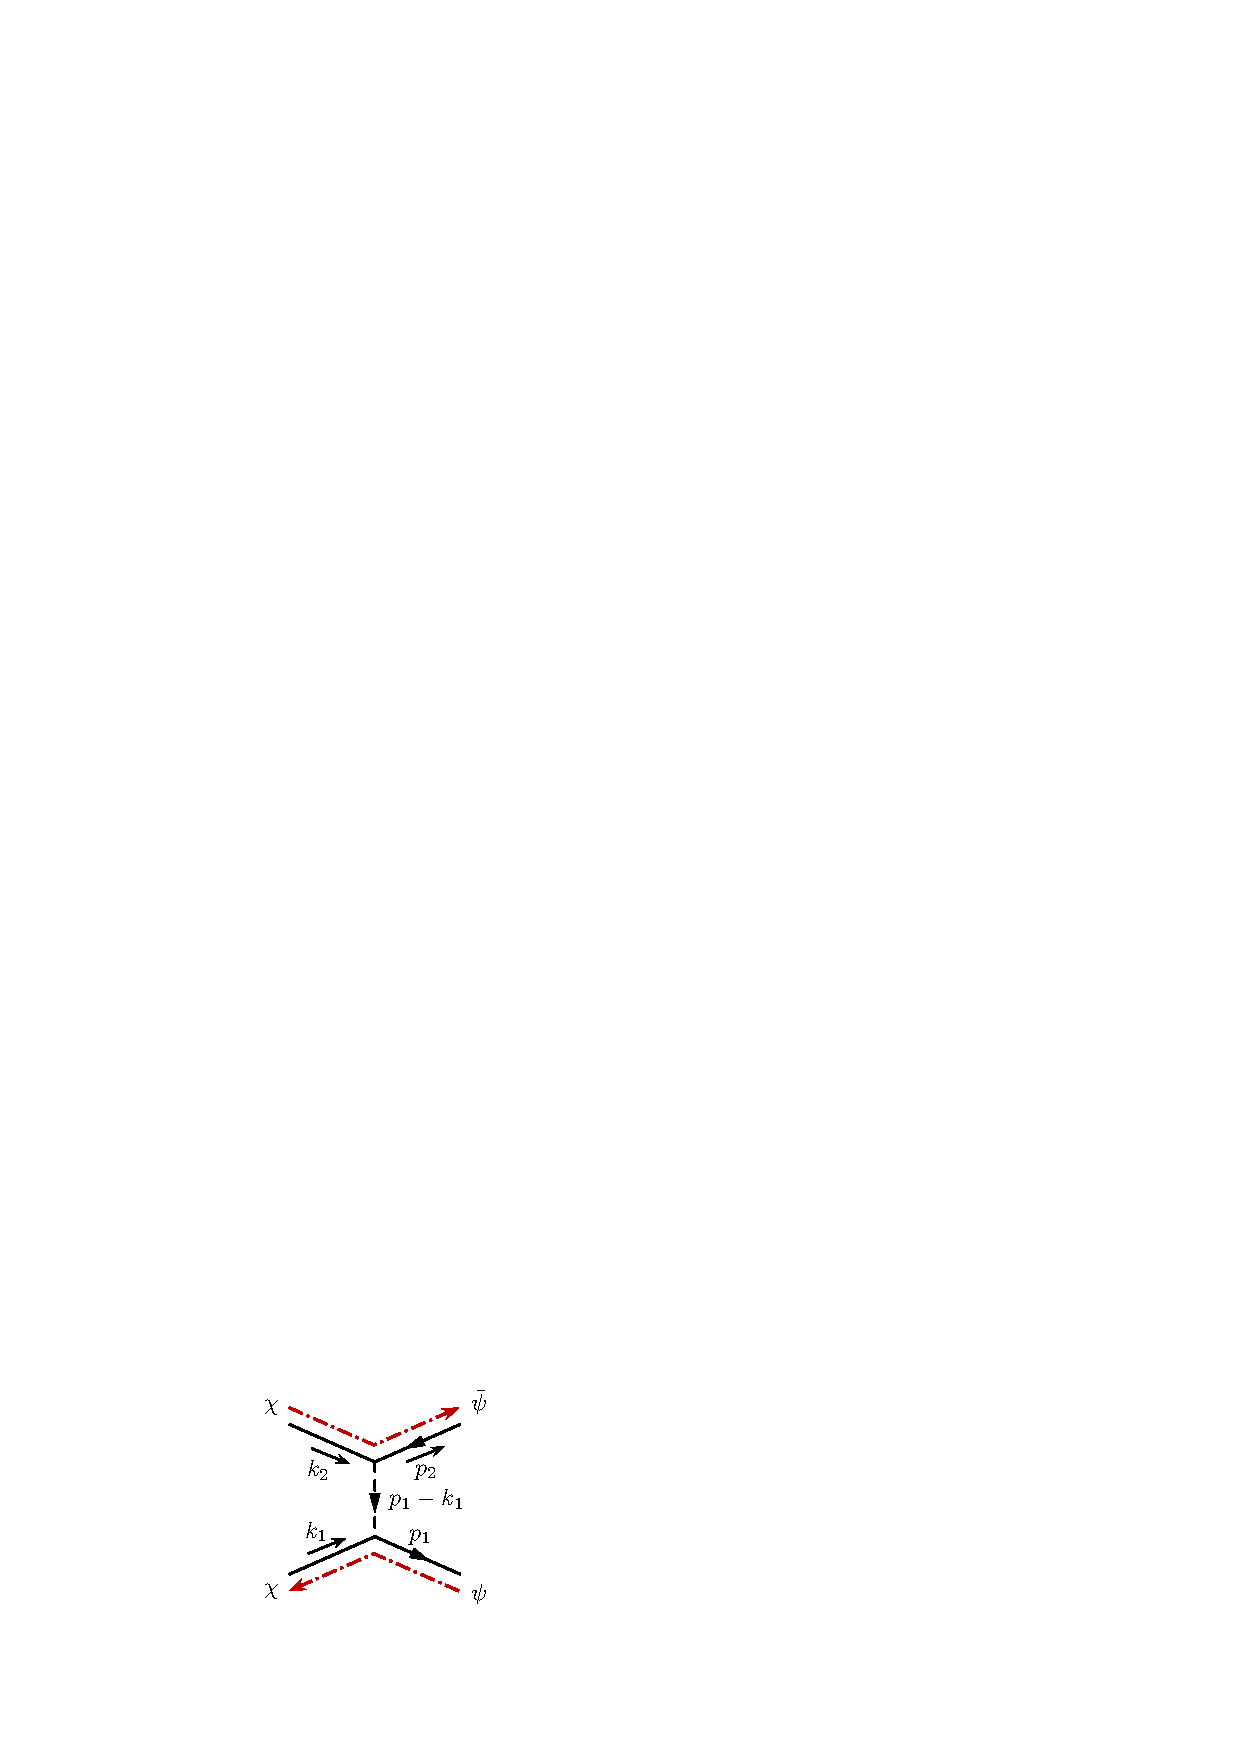
\includegraphics[width=3cm]{figs/fig25.pdf}}=\bar{v}(k_1)(\mathrm{i}\kappa\Gamma_2^\mathrm{C})v(p_1)\frac{\mathrm{i}}{(p_1-k_1)^2-m_\phi^2}\bar{u}(p_2)(\mathrm{i}\kappa\Gamma_1^\mathrm{C})u(k_2)\\
		&=-\frac{\mathrm{i}\kappa^2}{t-m_\phi^2}\bar{v}(k_1)\Gamma_2^\mathrm{C}v(p_1)\bar{u}(p_2)\Gamma_1^\mathrm{C}u(k_2)
	\end{aligned}
\end{equation}
\begin{equation}
	\begin{aligned}
	\mathrm{i}\tilde{\mathcal{A}}_u&=\parbox[c]{3cm}{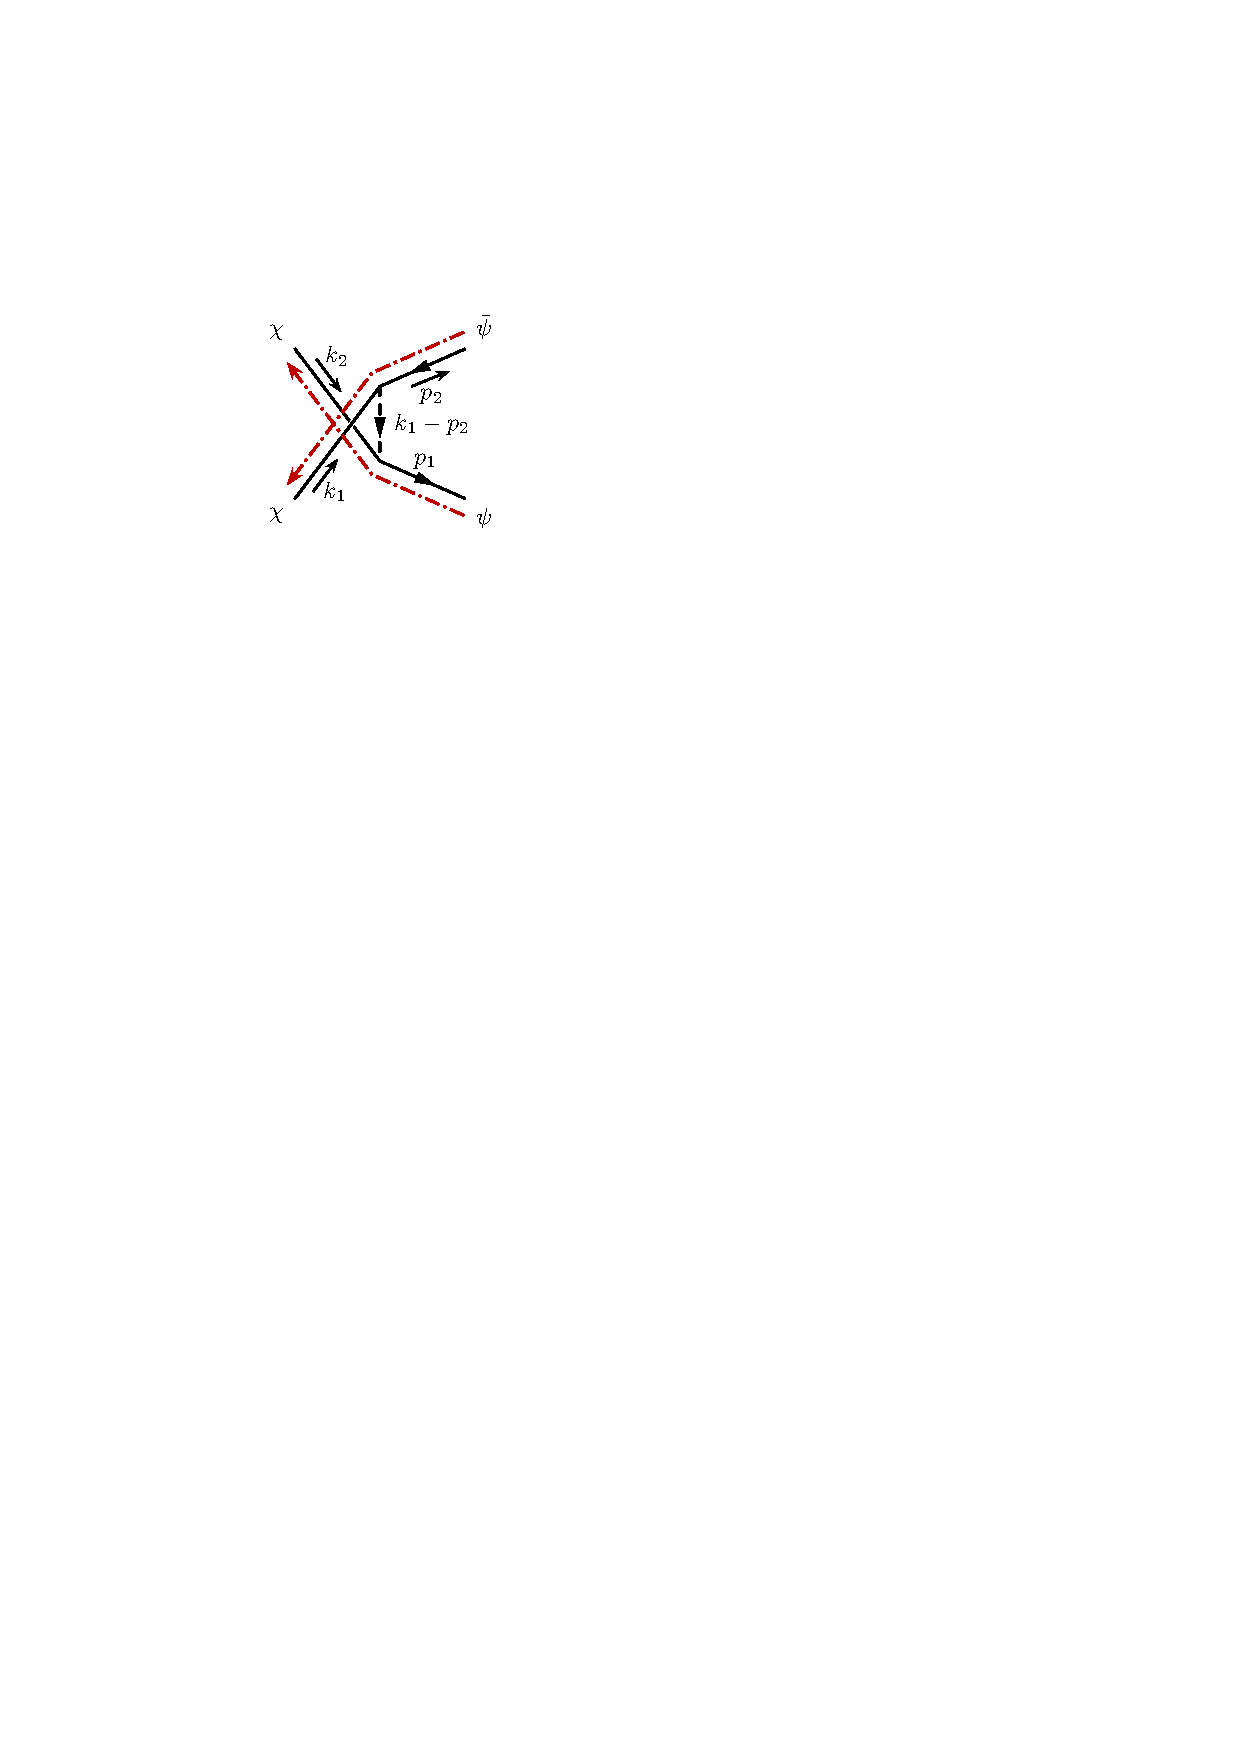
\includegraphics[width=3cm]{figs/fig26.pdf}}=\bar{v}(k_1)(\mathrm{i}\kappa\Gamma_1)v(p_2)\frac{\mathrm{i}}{(k_1-p_2)^2-m_\phi^2}\bar{v}(k_2)(\mathrm{i}\kappa\Gamma_2^\mathrm{C})v(p_1)\\
	&=-\frac{\mathrm{i}\kappa^2}{u-m_\phi^2}\bar{v}(k_1)\Gamma_1v(p_2)\bar{v}(k_2)\Gamma_2^\mathrm{C}v(p_1)
\end{aligned}
\end{equation}
显然这两个的相对符号为正,根据前面的思路\ref{A.5}不难证明两种计算方式得到的结果是等价的。

对于只有Dirac旋量,不含Majorana旋量的费曼规则,上面的所有方法完全适用,只是这个时候就把费米子流取为和$U(1)$流同向,不用额外画出来。
\subsection{拉氏量顶点项中含有偏导数}
原则上所有的费曼规则的构造都可以回到路径积分或者正则量子化本身上去导出,我们不care这些原理,直接给结论怎么通过拉氏量看出来。从现在开始,度规约定回到$(-+++)$。

含有偏导数的理论的代表是标量QED,这是复标量场(实标量场没有$U(1)$流来耦合)和电磁场的耦合:
\begin{equation}
	\mathcal{L}_{\text{int}}=ieA^\mu[(\partial_\mu\varphi^\dagger)\varphi-\varphi^\dagger\partial_\mu\varphi]-e^2A^\mu A_\mu\varphi^\dagger\varphi-\frac14\lambda(\varphi^\dagger\varphi)^2
\end{equation}
以及非阿贝YM理论,我们以标量QED为例,显然有下面的三个顶点:
\begin{figure}[htbp]
	\centering
	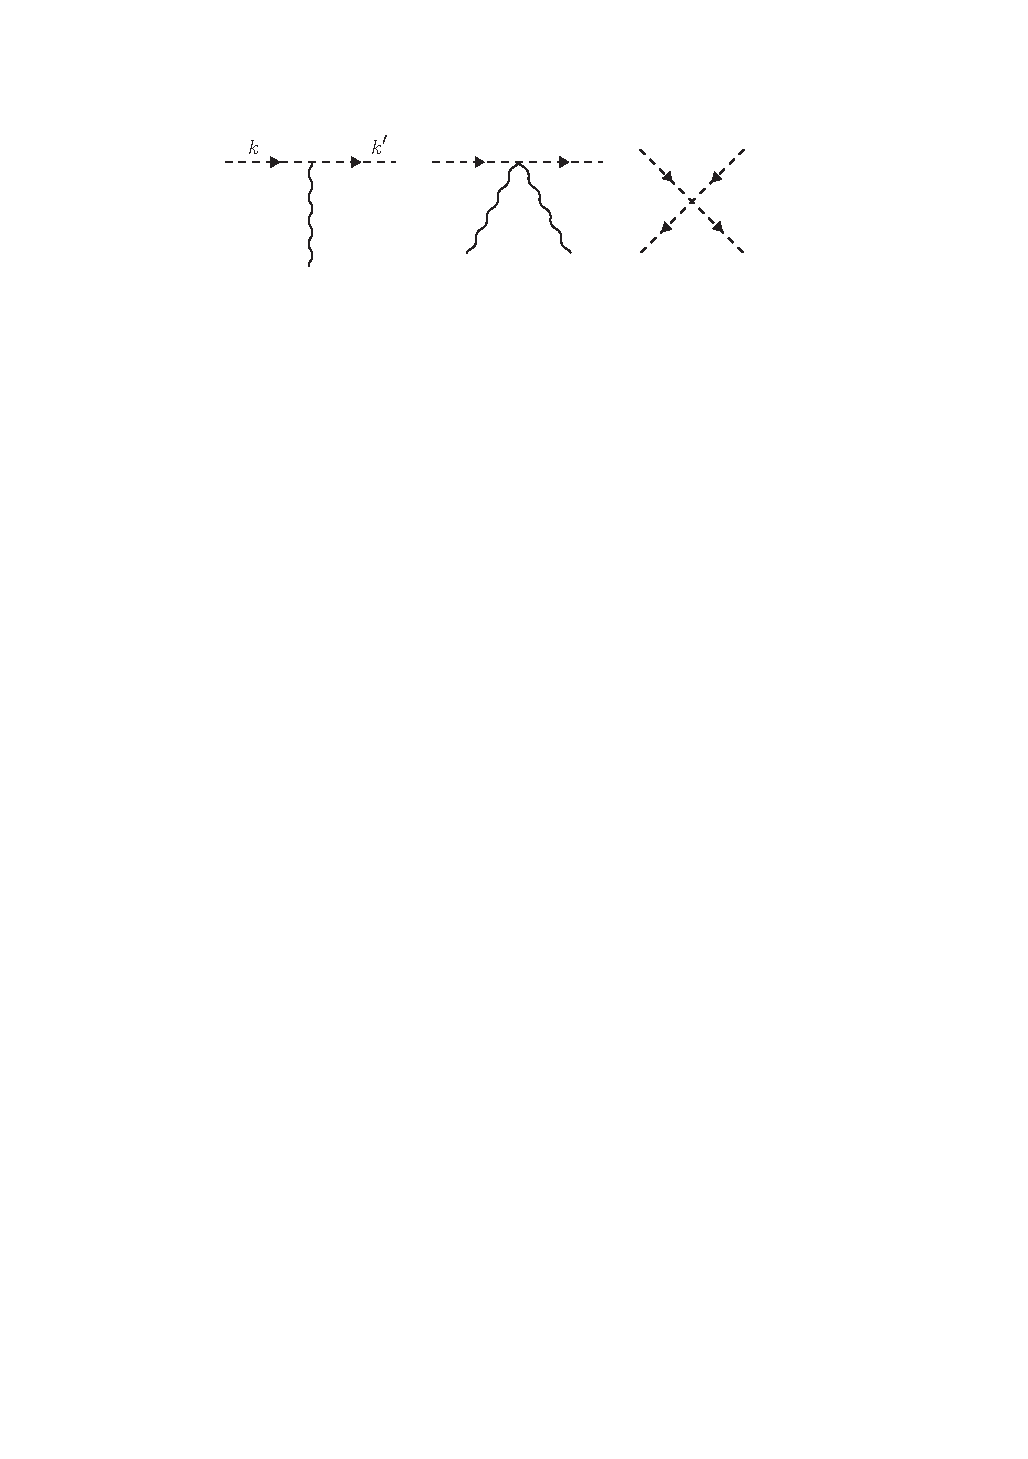
\includegraphics{figs/fig27.pdf}
	\caption{标量QED顶点}
	\label{sqed}
\end{figure}
由于费曼规则与光子外线无关,所以没有把光子的动量箭头标出来,另外我们选取了动量箭头和$U(1)$箭头相同,也可以不同,适当的地方加个负号就好。后面的两个图都不含有偏导数项,我们着重考虑第一个图。搞清楚这一构造最简单的方法其实是从正则量子化,从位置空间的费曼规则出发,总结为表\ref{A.7},其中光子和胶子是一样的,只需要加个色因子就好\footnote{$A^\mu$不带螺旋度指标,因为正则量子化框架下它是$a^\dagger_\lambda$的求和,但是QCD里$A^{\mu a}$要带色指标,带哪个色指标就负责产生湮灭哪个色指标的胶子。但是外线规则与带的哪个色无关,因为极化矢量都是一样的。}。表中给的都是对外线在壳情况的缩并,不在壳情况要替换成传播子,不过就推导顶点规则而言,我们完全可以假设所有外线都是在壳的。
\begin{table}
	\centering
	\begin{tabular}{cc}
		\toprule
		费曼图& 缩并规则  \\
		\midrule
		\makecell*[c]{
			\begin{tikzpicture}
				\begin{feynman}
				\vertex (a) {\(\phi\)};
				\vertex[right=2cm of a] (b);
				\diagram*{
				(a) -- [charged scalar,momentum=\(p\)] (b) ,};
				\fill (b) circle (2pt);
				\node[right=2pt] at (b) {$x$};
				\end{feynman}
			\end{tikzpicture}
		} & \makecell*[c]{$\left<0\right|\wick{\c{\phi}(x)|\c{\mathbf{p}}^{+}\rangle}=\left<0\right|\phi^{\left(+\right)}(x)\left|\mathbf{p}^{+}\right>=\mathrm{e}^{+\mathrm{i}p\cdot x}$}  \\
		\makecell*[c]{
			\begin{tikzpicture}
				\begin{feynman}
					\vertex (a) {\(\bar\phi\)};
					\vertex[right=2cm of a] (b);
					\diagram*{
						(a) -- [anti charged scalar,momentum=\(p\)] (b) ,};
					\fill (b) circle (2pt);
					\node [right=2pt] at (b) {$x$};
				\end{feynman}
			\end{tikzpicture}
		} & \makecell{$\left<0\right|\wick{\c{\phi}^\dagger(x)|\c{\mathbf{p}}^{-}\rangle}=\left<0\right|\phi^{\dagger\left(+\right)}(x)\left|\mathbf{p}^{-}\right>=\mathrm{e}^{+\mathrm{i}p\cdot x}$}   \\
		 \makecell*[c]{
		 	\begin{tikzpicture}
		 		\begin{feynman}
		 			\vertex (a) {\(\phi\)};
		 			\vertex[right=2cm of a] (b);
		 			\diagram*{
		 				(a) -- [anti charged scalar,reversed momentum=\(p\)] (b) ,};
		 			\fill (b) circle (2pt);
		 			\node [right=2pt] at (b) {$x$};
		 		\end{feynman}
		 	\end{tikzpicture}
		 }& \makecell*[c]{$\wick{\langle\c{\mathbf{p}}^{+}|\c{\phi}^{\dagger}(x)}\left|0\right\rangle=\left\langle\mathbf{p}^{+}\right|\phi^{\dagger(-)}(x)\left|0\right\rangle=\mathrm{e}^{-\mathrm{i}p\cdot x}$}  \\
		\makecell*[c]{
			\begin{tikzpicture}
				\begin{feynman}
					\vertex (a) {\(\bar \phi\)};
					\vertex[right=2cm of a] (b);
					\diagram*{
						(a) -- [ charged scalar,reversed momentum=\(p\)] (b) ,};
					\fill (b) circle (2pt);
					\node [right=2pt] at (b) {$x$};
				\end{feynman}
			\end{tikzpicture}
		}	 & \makecell*[c]{$\wick{\langle\c{\mathbf{p}}^{-}|\c{\phi}(x)}\left|0\right\rangle=\left\langle\mathbf{p}^{-}\right|\phi^{(-)}(x)\left|0\right\rangle=\mathrm{e}^{-\mathrm{i}p\cdot x}$}  \\
		\makecell*[c]{
			\begin{tikzpicture}
				\begin{feynman}
					\vertex (a) {\(A^\mu\)};
					\vertex[right=2cm of a] (b);
					\diagram*{
						(a) -- [photon, momentum=\(p^{(\lambda)}\)] (b) ,};
					\fill (b) circle (2pt);
					\node [right=2pt] at (b) {$x$};
				\end{feynman}
			\end{tikzpicture}
		}	 & \makecell*[c]{$\left\langle0\right|\wick{\c {A}^{\mu}(x)|\c{\mathbf{p}},\lambda\rangle}=\left\langle0\right|A^{\mu(+)}(x)\left|\mathbf{p},\lambda\right\rangle=\varepsilon^{\mu}(\mathbf{p},\lambda)\mathrm{e}^{+\mathrm{i}p\cdot x}$} \\
		\makecell*[c]{
			\begin{tikzpicture}
				\begin{feynman}
					\vertex (a) {\(A^{\mu}\)};
					\vertex[right=2cm of a] (b);
					\diagram*{
						(a) -- [photon,reversed momentum=\(p^{(\lambda)}\)] (b) ,};
					\fill (b) circle (2pt);
					\node [right=2pt] at (b) {$x$};
				\end{feynman}
			\end{tikzpicture}
		} & \makecell*[c]{$\wick{\langle\c{\mathbf{p}},\lambda|\c{A}^{\mu}(x)}\left|0\right\rangle=\left\langle\mathbf{p},\lambda\right|A^{\mu(-)}(x)\left|0\right\rangle=\varepsilon^{\mu*}(\mathbf{p},\lambda)\mathrm{e}^{-\mathrm{i}p\cdot x}$} \\
		\makecell*[c]{
			\begin{tikzpicture}
				\begin{feynman}
					\vertex (a) {\(A^{\mu b}\)};
					\vertex[right=2cm of a] (b);
					\diagram*{
						(a) -- [gluon, momentum=\(p^{(\lambda)}_a\)] (b) ,};
					\fill (b) circle (2pt);
					\node [right=2pt] at (b) {$x$};
				\end{feynman}
			\end{tikzpicture}
		}& \makecell*[c]{$\left\langle0\right|\wick{\c {A}^{\mu b}(x)|\c{\mathbf{p}},\lambda,a\rangle}=\left\langle0\right|A^{\mu(+)}(x)\left|\mathbf{p},\lambda\right\rangle=\delta^{ab}\varepsilon^{\mu}(\mathbf{p},\lambda)\mathrm{e}^{+\mathrm{i}p\cdot x}$}\\
		\makecell*[c]{
			\begin{tikzpicture}
				\begin{feynman}
					\vertex (a) {\(A^{\mu b}\)};
					\vertex[right=2cm of a] (b);
					\diagram*{
						(a) -- [gluon,reversed momentum=\(p^{(\lambda)}_a\)] (b) ,};
					\fill (b) circle (2pt);
					\node [right=2pt] at (b) {$x$};
				\end{feynman}
			\end{tikzpicture}
		}&\makecell*[c]{$\wick{\langle\c{\mathbf{p}},\lambda,a|\c{A}^{\mu b}(x)}\left|0\right\rangle=\left\langle\mathbf{p},\lambda\right|A^{\mu(-)}(x)\left|0\right\rangle=\delta^{ab}\varepsilon^{\mu*}(\mathbf{p},\lambda)\mathrm{e}^{-\mathrm{i}p\cdot x}$}\\
		\bottomrule
	\end{tabular}
	\caption{一般的外线缩并,这里上标$(\pm)$表示正反粒子,$p^{(\lambda)}_a$表示色指标为$a$,螺旋度为$\lambda$.图中没有的缩并项表明缩并后为0.}
	\label{A.7}
\end{table}

费曼图顶点的本质其实就是在$\bra{\text{out}}$和$\ket{\text{in}}$之间插入$e^{i\int d^4x\mathcal{H}_I}$后展开带来的那些“抱团”的场算符。第一个图按照我们的箭头约定是$\ket{k}$的正粒子到$\ket{k^\prime}$的正粒子的顶角修正,而且关注的是最低阶的树图顶角,所以考虑$e$指数展开的线性项就好了,也就是下面两项修正,计算所有可能的场与外线的缩并:
\begin{equation}
	\begin{aligned}
		\wick{\langle \c k'|(\partial_\mu\c\varphi^\dagger)}\wick{\c\varphi|\c k\rangle}&=\partial_\mu e^{-ik^\prime x}\cdot{e}^{ikx}=-ik'_\mu e^{-i(k'-k)x}\\
		\wick{\langle\c k'|\c\varphi^\dagger}\partial_\mu\wick{\c\varphi|\c k\rangle}&= e^{-ik^\prime x}\cdot\partial_\mu{e}^{ikx}=+ik_\mu e^{-i(k'-k)x}
	\end{aligned}
\end{equation}
把两者相减,并且去掉本身外线会带来的那些$e$指数的项,我们就得到了纯的顶点的贡献:$i(ie)[(-ik_{\mu}')-(ik_{\mu})]=ie(k+k')_{\mu}$。\footnote{按照惯例,顶角函数多乘了个$i$}

而且上面的缩并和对应的表\ref{A.7}中的费曼图构造出来的顶点图恰好就是图\ref{sqed}第一幅图。所以上面的构造方法是有效的,而且一定程度上我们也说明了这种方法的原因。注意到上面的推导中我们完全可以在入射或者出射态中加入$\ket{\gamma}$,也就是光子项,拉氏量里$A^\mu$和它缩并的作用就是单纯的一个$e$指数配上极化矢量,这没有任何的顶点贡献,纯粹来自于粒子在壳的贡献,所以印证了前面所说的不需要care光子。这也说明了为何构造feynman图顶点项时,在不含导数项的时候,就是把所有的场全部抽走,前面的对称因子也抽走带来的项。可见虽然我们这里讨论的只是含偏导项的feynman图顶点构造,但这完全是一般的做法,某种程度上说,虽然从路径积分看出费曼图本身数学上非常清晰舒服,但构造费曼规则而言,正则量子化这种形式更直观。

如果把左边的粒子也改成出射,也就是说把动量箭头反向,这个时候是一个出射的动量为$k$的反粒子$\bra{\bar k}$,对应的费曼规则由下式计算:
\begin{equation}
		\begin{aligned}
			\wick{\langle \c1 k',\c2 {\bar {k}}|(\partial_\mu\c1\varphi^\dagger)\c2\varphi| 0\rangle}&=\partial_\mu e^{-ik^\prime x}\cdot{e}^{-ikx}=-ik'_\mu e^{-i(k'+k)x}\\
			\wick{\langle\c1 k',\c2{\bar k}|\c1\varphi^\dagger\partial_\mu\c2\varphi|0\rangle}
			&= e^{-ik^\prime x}\cdot\partial_\mu{e}^{-ikx}=-ik_\mu e^{-i(k'+k)x}
		\end{aligned}
\end{equation}
两式相减就得到结果$ie(k'-k)_{\mu}$。从上面的推导可以看出,确实就是前面说的把$k\to- k$,也确实就是动量参考方向变了,而且上面公式对应的图表示也是和\ref{sqed}对的上的。
\begin{example}
	QCD的三胶子顶点是个完美的练习,对应的拉氏量为:
	\begin{equation}
		\mathcal{L}_{\text{YM}}\supset-gf^{abe}A^{a\mu}A^{b\nu}\partial_{\mu}A_{\nu}^{e}
	\end{equation}
	正确答案如下:
	\begin{equation}\label{A.14}
		\mathrm{i}\cdot\parbox[c]{3cm}{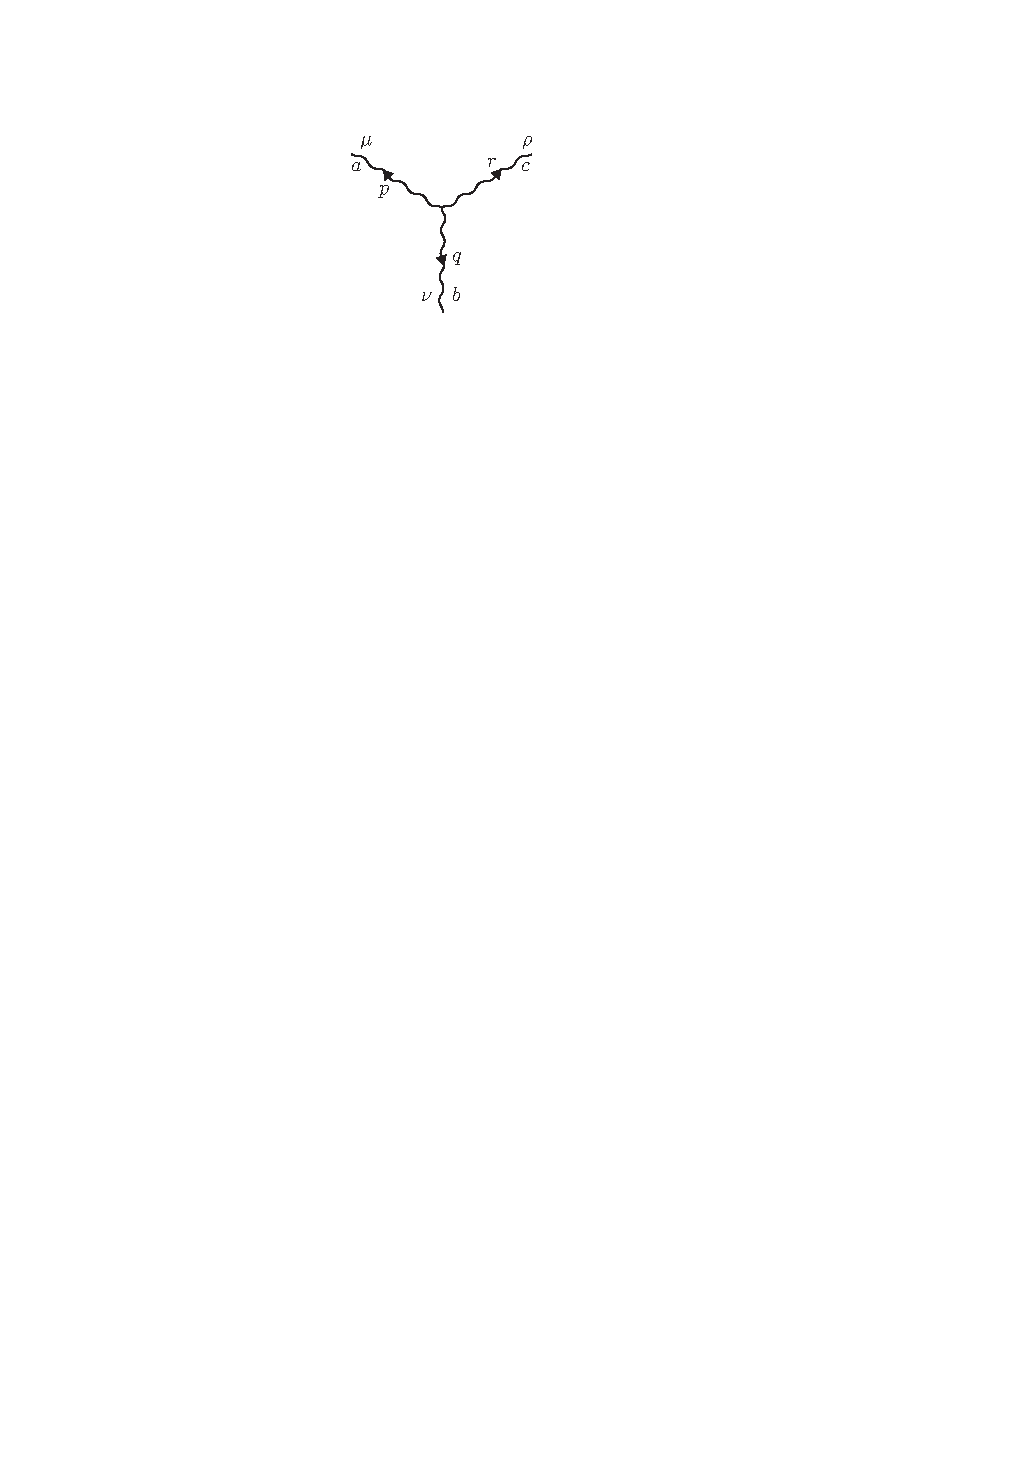
\includegraphics[width=3cm]{figs/fig28.pdf}}=gf^{abc}[(q-r)_{\mu}g_{\nu\rho}+(r-p)_{\nu}g_{\rho\mu}+(p-q)_{\rho}g_{\mu\nu}]
	\end{equation}
	同样也是用场进行缩并就好,主要要计算所有可能的缩并,详细计算过程如下:
	\begin{equation}
		\begin{aligned}
			&-ig\langle {p}^a,{q}^b,{r}^c|f^{def}{A}^{d\mu}{A}^{e\nu}\partial_\mu {A}_\nu^f\ket{0}\\
			=&-ig\wick{\langle\c1 {p}^a,\c2{q}^b,\c3{r}^c|f^{def}\c1{A}^{d\mu}\c2{A}^{e\nu}\partial_\mu \c3{A}_\nu^f}\ket{0}-ig\wick{\langle\c1 {p}^a,\c3{q}^b,\c2{r}^c|f^{def}\c1{A}^{d\mu}\c2{A}^{e\nu}\partial_\mu \c3{A}_\nu^f}\ket{0}\\
			&-ig\wick{\langle\c2 {p}^a,\c1{q}^b,\c3{r}^c|f^{def}\c1{A}^{d\mu}\c2{A}^{e\nu}\partial_\mu \c3{A}_\nu^f}\ket{0}-ig\wick{\langle\c2 {p}^a,\c3{q}^b,\c1{r}^c|f^{def}\c1{A}^{d\mu}\c2{A}^{e\nu}\partial_\mu \c3{A}_\nu^f}\ket{0}\\
			&-ig\wick{\langle\c3 {p}^a,\c1{q}^b,\c2{r}^c|f^{def}\c1{A}^{d\mu}\c2{A}^{e\nu}\partial_\mu \c3{A}_\nu^f}\ket{0}-ig\wick{\langle\c3 {p}^a,\c2{q}^b,\c1{r}^c|f^{def}\c1{A}^{d\mu}\c2{A}^{e\nu}\partial_\mu \c3{A}_\nu^f}\ket{0}\\
			=&-igf^{def}\delta^{ad}\delta^{be}\delta^{cf}(-ir_\mu)\epsilon_{\lambda^a}^{*\mu}\epsilon_{\lambda^b}^{*\nu}\epsilon^{*}_{\lambda^c\nu}\mathrm{e}^{i(p+q+r)\cdot x}-igf^{def}\delta^{ad}\delta^{bf}\delta^{ce}(-iq_\mu)\epsilon_{\lambda^a}^{*\mu}\epsilon_{\lambda^c}^{*\nu}\epsilon^{*}_{\lambda^b\nu}\mathrm{e}^{i(p+q+r)\cdot x}\\
			&-igf^{def}\delta^{ae}\delta^{bd}\delta^{cf}(-ir_\mu)\epsilon_{\lambda^b}^{*\mu}\epsilon_{\lambda^a}^{*\nu}\epsilon^{*}_{\lambda^c\nu}\mathrm{e}^{i(p+q+r)\cdot x}+\cdots\\
			=&gf^{abc}\left[(q-r)_\mu g_{\nu\rho}+r_\nu g_{\rho\mu}\cdots\right]\cdot\left[\epsilon_{\lambda^a}^{*\mu}\epsilon_{\lambda^b}^{*\nu}\epsilon^{*\rho}_{\lambda^c}\mathrm{e}^{i(p+q+r)\cdot x}\right]\\
		\end{aligned}
	\end{equation}
	根据外线本身就固有的因子$\epsilon_{\lambda^a}^{*\mu}\epsilon_{\lambda^b}^{*\nu}\epsilon^{*\rho}_{\lambda^c}\mathrm{e}^{i(p+q+r)\cdot x}$,合理对哑指标进行操作后就不难得到上面这个式子,其中还用到了$SU(3)$的结构常数是全反对称的。去掉外线带来的因子后就得到了顶点项,显然与\ref{A.14}一致。
\end{example}

还有一个费曼规则疑难杂症,就是矩阵模型的费曼规则,要使用所谓的double line表示,这部分有两种想法,一是回到色因子的图规则构造,然后配以$T^a$得到${A^i}_j$的费曼规则。第二种方法就是直接从矩阵模型本身出发,注意到double line配对与矩阵乘法关系,还是按照前面的缩并的思想,把每个矩阵元${A^i}_j$单独看成一个场来构造费曼规则。

